%%%%%%%%%%%%%%%%%%%%%%%%%%%%%%%%%%%%%%%%%
% Template
% LaTeX Template
% Version 1.0 (December 8 2014)
%
% This template has been downloaded from:
% http://www.LaTeXTemplates.com
%
% Original author:
% Brandon Fryslie
% With extensive modifications by:
% Vel (vel@latextemplates.com)
%
% License:
% CC BY-NC-SA 3.0 (http://creativecommons.org/licenses/by-nc-sa/3.0/)
%
% Authors:
% Sabbir Ahmed
%
%%%%%%%%%%%%%%%%%%%%%%%%%%%%%%%%%%%%%%%%%

\documentclass[paper=usletter, fontsize=12pt]{article}
%%%%%%%%%%%%%%%%%%%%%%%%%%%%%%%%%%%%%%%%%
% Contract Structural Definitions File Version 1.0 (December 8 2014)
%
% Created by: Vel (vel@latextemplates.com)
% 
% This file has been downloaded from: http://www.LaTeXTemplates.com
%
% License: CC BY-NC-SA 3.0 (http://creativecommons.org/licenses/by-nc-sa/3.0/)
%
%%%%%%%%%%%%%%%%%%%%%%%%%%%%%%%%%%%%%%%%%

\usepackage{geometry} % Required to modify the page layout
\usepackage{multicol}
\usepackage{amsmath}
\usepackage{amssymb}

\usepackage[pdftex]{graphicx}
\usepackage{wrapfig}
\usepackage[font=scriptsize, labelfont=bf]{caption}
\usepackage[utf8]{inputenc} % Required for including letters with accents
\usepackage[T1]{fontenc} % Use 8-bit encoding that has 256 glyphs

\usepackage{avant} % Use the Avantgarde font for headings
\usepackage{courier}
\usepackage{xparse}
\usepackage{xcolor}
\usepackage{listings}  % for code verbatim and console outputs

\setlength{\textwidth}{16cm} % Width of the text on the page
\setlength{\textheight}{23cm} % Height of the text on the page
\setlength{\oddsidemargin}{0cm} % Width of the margin - negative to move text left, positive to move it right
\setlength{\topmargin}{-1.25cm} % Reduce the top margin

\setlength{\parindent}{0mm} % Don't indent paragraphs
\setlength{\parskip}{2.5mm} % Whitespace between paragraphs
\renewcommand{\baselinestretch}{1.5}

\definecolor{green}{rgb}{0.18, 0.55, 0.34}

\graphicspath{ {figures/} }
\captionsetup[table]{skip=10pt}

\lstset{language=C, keywordstyle={\bfseries \color{black}}}

% defines algorithm counter for chapter-level
\newcounter{nalg}[section]

%defines appearance of the algorithm counter
\renewcommand{\thenalg}{\thesection .\arabic{nalg}}

% defines a new caption label as Algorithm x.y
\DeclareCaptionLabelFormat{algocaption}{Algorithm \thenalg}

% defines the algorithm listing environment
\lstnewenvironment{pseudocode}[1][] {
    \refstepcounter{nalg}  % increments algorithm number
    \captionsetup{font=normalsize, labelformat=algocaption, labelsep=colon}
    \lstset{
        breaklines=true,
        mathescape=true,
        numbers=left,
        numberstyle=\scriptsize,
        basicstyle=\footnotesize\ttfamily,
        keywordstyle=\color{black}\bfseries,
        keywords={input, output, return, parallel, function, for, to, in, if,
        else, foreach, while, and, or, new, print},
        xleftmargin=.04\textwidth,
        #1
    }
}{}

\renewcommand{\familydefault}{\sfdefault}  % default font for entire document
 % specifies the document layout and style
\usepackage{tikz}
\usepackage{xcolor}
\usetikzlibrary{arrows.meta}

\begin{document}

    \documentinfo{\today}{10}

    \begin{itemize}

        \item[\textbf{3.6}]
        \begin{itemize}

            \item[\textbf{5}] Show that no proper subgroup of $S_4$ contains
            both $(1, 2, 3, 4)$ and $(1, 2)$.
            \begin{proof}

                Suppose $H \le S_4$ with the permutations $(1 \ 2 \ 3 \ 4)$ and
                $(1 \ 2)$\\
                \begin{equation*}
                    \left(\begin{tabular}{cccc}
                            1 & 2 & 3 & 4 \\
                            2 & 3 & 4 & 1
                    \end{tabular}\right),
                    \left(\begin{tabular}{cccc}
                            1 & 2 & 3 & 4 \\
                            2 & 1 & 3 & 4
                    \end{tabular}\right)
                \end{equation*}
                Their product would yield
                \begin{equation*}
                    \left(\begin{tabular}{cccc}
                            1 & 2 & 3 & 4 \\
                            1 & 3 & 4 & 2
                    \end{tabular}\right) = S_4
                \end{equation*}
                Therefore, $H$ is not a proper subgroup of $S_4$ by
                contradiction \qedhere

            \end{proof}

            \item[\textbf{9}] A rigid motion of a cube can be thought of either
            as a permutation of its eight vertices or as a permutation of its
            six sides. Find a rigid motion of the cube that has order 3, and
            express the permutation that represents it in both ways, as a
            permutation on eight elements and as a permutation on six elements.
            \begin{proof}

                \begin{figure}[h]
                    \centering
                    \caption{Cube of order 3}
                    \begin{tikzpicture}
                        \node (C) at (0,0,2) {1};
                        \node (G) at (2,0,2) {2};
                        \node (F) at (2,2,2) {3};
                        \node (B) at (0,2,2) {4};
                        \node (O) at (0,0,0) {5};
                        \node (D) at (2,0,0) {6};
                        \node (E) at (2,2,0) {7};
                        \node (A) at (0,2,0) {8};

                        \draw(-1,1,2) node{front};
                        \draw(1,2,1) node{top};
                        \draw(2,1,1) node{right};
                        \draw[gray!80](1,0,1) node{bottom};
                        \draw[gray!80](0,1,1) node{left};
                        \draw[gray!80](3,1,0) node{back};

                        \draw (O) -- (C) -- (G) -- (D) -- cycle;% Bottom Face
                        \draw (O) -- (A) -- (E) -- (D) -- cycle;% Back Face
                        \draw (O) -- (A) -- (B) -- (C) -- cycle;% Left Face
                        \draw (O) -- (D) -- (E) -- (A) -- cycle;% Left Face
                        \draw (D) -- (E) -- (F) -- (G) -- cycle;% Right Face
                        \draw (C) -- (B) -- (F) -- (G) -- cycle;% Front Face
                        \draw (A) -- (B) -- (F) -- (E) -- cycle;% Top Face
                    \end{tikzpicture}
                \end{figure}
                Rigid motion of order 3 will be rotating the cube about a vector passing through $(1,7)$ 120$^\circ$ \\
                The permutation of the eight vertices are $(2,4,5)(3,8,6)$ \\
                and the sides are (front, left, back)(top, back, right) \qedhere

            \end{proof}

            \item[\textbf{10}] Show that the following matrices form a subgroup
            of $\gl_2(\mathbb{C})$ isomorphic to $D_4$:
            \begin{equation*}
                \pm\left[\begin{tabular}{cc}
                            1 & 0 \\
                            0 & 1
                \end{tabular}\right],
                \pm\left[\begin{tabular}{cc}
                            i & 0 \\
                            0 & -i
                \end{tabular}\right],
                \pm\left[\begin{tabular}{cc}
                            0 & 1 \\
                            1 & 0
                \end{tabular}\right],
                \pm\left[\begin{tabular}{cc}
                            0 & i \\
                            -i & 0
                \end{tabular}\right]
            \end{equation*}
            \begin{proof}

                Let $a = \left[\begin{tabular}{cc}
                           $i$ & 0 \\
                            0 & $-i$
                \end{tabular}\right]$ and $b = \left[\begin{tabular}{cc}
                            0 & 1 \\
                            1 & 0
                \end{tabular}\right]$\\

                Then,
                \salign{1}
                \begin{align*}
                    a^2 & = \left(\left[\begin{tabular}{cc}
                           $i$ & 0 \\
                            0 & $-i$
                    \end{tabular}\right]\right)^2 = \left[\begin{tabular}{cc}
                            -1 & 0 \\
                            0 & -1
                    \end{tabular}\right]\\
                    a^3 & = \left(\left[\begin{tabular}{cc}
                           $i$ & 0 \\
                            0 & $-i$
                    \end{tabular}\right]\right)^3 = \left[\begin{tabular}{cc}
                            $-i$ & 0 \\
                            0 & $i$
                    \end{tabular}\right]\\
                    a^4 & = \left(\left[\begin{tabular}{cc}
                           $i$ & 0 \\
                            0 & $-i$
                    \end{tabular}\right]\right)^4 = \left[\begin{tabular}{cc}
                            1 & 0 \\
                            0 & 1
                    \end{tabular}\right]\\
                    b^2 & = \left(\left[\begin{tabular}{cc}
                            0 & 1 \\
                            1 & 0
                    \end{tabular}\right]\right)^2 = \left[\begin{tabular}{cc}
                            1 & 0 \\
                            0 & 1
                    \end{tabular}\right]\\
                    ab & = \left[\begin{tabular}{cc}
                           $i$ & 0 \\
                            0 & $-i$
                    \end{tabular}\right]
                    \left[\begin{tabular}{cc}
                            0 & 1 \\
                            1 & 0
                    \end{tabular}\right] = \left[\begin{tabular}{cc}
                            0 & $i$ \\
                            $-i$ & 0
                    \end{tabular}\right]\\
                    a^2b & = \left[\begin{tabular}{cc}
                            -1 & 0 \\
                            0 & -1
                    \end{tabular}\right]
                    \left[\begin{tabular}{cc}
                            0 & 1 \\
                            1 & 0
                    \end{tabular}\right] = \left[\begin{tabular}{cc}
                            0 & -1 \\
                            -1 & 0
                    \end{tabular}\right]\\
                    a^3b & = \left[\begin{tabular}{cc}
                            $i$ & 0 \\
                            0 & $-i$
                    \end{tabular}\right]
                    \left[\begin{tabular}{cc}
                            0 & 1 \\
                            1 & 0
                    \end{tabular}\right] = \left[\begin{tabular}{cc}
                            0 & $-i$ \\
                            $i$ & 0
                    \end{tabular}\right]
                \end{align*}
                \endgroup

                Which forms the set
                \begin{align*}
                    \gl_2(\mathbb{C}) & = \{e,a,a^2,a^3,b,ab,a^2b,a^3b\}, \text{ with } a^4=b^2=e, \ ba=a^{-1}b\\
                    & \cong D_4 \qedhere
                \end{align*}

            \end{proof}

            \item[\textbf{15}]
            \begin{enumerate}[label=\textbf{(\alph*)}]

                \item Show that $A_4=\{\sigma \in S_4 \mid \sigma = \tau^2
                \text{ for some } \tau \in S_4\}$
                \begin{proof}
                \end{proof}

                \item Show that $A_5=\{\sigma \in S_5 \mid \sigma = \tau^2
                \text{ for some } \tau \in S_5\}$
                \begin{proof}
                \end{proof}

                \item Show that $A_6=\{\sigma \in S_6 \mid \sigma = \tau^2
                \text{ for some } \tau \in S_6\}$
                \begin{proof}
                \end{proof}

                \item What can you say about $A_n$ if $n>6$?
                \begin{proof}
                \end{proof}

            \end{enumerate}

            \item[\textbf{17}] For any elements $\sigma, \tau \in S_n$, show
            that $\sigma\tau\sigma^{-1}\tau^{-1}\in A_n$.
            \begin{proof}

                Let $\sigma,\tau \in S_n$ be the products of $m$ and $n$
                transpositions respectively\\
                Thus, $\sigma^{-1},\tau^{-1} \in S_n$ are also the products of
                $m$ and $n$ transpositions\\
                Therefore, $\sigma\tau\sigma^{-1}\tau^{-1}$ is a product of
                $m+n+m+n=2(m+n)$ transpositions\\
                Since $2 \mid 2(m+n)$, $\sigma\tau\sigma^{-1}\tau^{-1} \in A_n$
                \qedhere

            \end{proof}

            \item[\textbf{21}] Find the center of the dihedral group $D_n$. \\
            \textit{Hint:} Consider two cases, depending on whether $n$ is odd
            or even.
            \begin{proof}

                The center of a group is the subgroup consisting of all the
                elements that commute with every other element in the group\\
                The group $D_1$ is $\mathbb{Z}/2\mathbb{Z}$, and $D_2$ is
                $\mathbb{Z}/2\mathbb{Z}\times\mathbb{Z}/2\mathbb{Z}$ \\
                Let $n > 2$, and assume $yx^k$ is in the center,\\
                That is, $yx^k$ must commute with $x$\\
                Then,
                \begin{equation*}
                    xyx^kx^{-1} = yx^{k-2} = yx^k
                \end{equation*}
                Which implies, $2 \equiv 0 \Mod{n}$, (contradiction)\\
                Therefore, $x^k$ is in the center iff $2k \equiv 0 \Mod{n}$\\
                If $n$ is odd, then the center of $D_{2m+1}$ is $\{e\}$\\
                If $n$ is even, then the center of $D_{2m}$ is $\{e,x^m\}$ \qedhere

            \end{proof}

            \item[\textbf{24}] Show that the product of two transpositions is
            one of (i) the identity; (ii) a 3-cycle; (iii) a product of two
            (non-disjoint) 3-cycles. Deduce that every element of $A_n$ can be
            written as a product of 3-cycles.
            \begin{proof}

                Consider $\sigma = (1,2,3,4)$\\
                (i) For identity,
                \begin{equation*}
                    (1,2)(1,2) = (1)
                \end{equation*}

                (ii) For a 3-cycle,
                \begin{equation*}
                    (1,2)(2,3) = (1,3,2)
                \end{equation*}

                (iii) For a product of two (non-disjoint) 3-cycles,
                \begin{equation*}
                    (1,2)(3,4) = (1,2,3)(1,4,3)
                \end{equation*}

                Since $A_n$ is a set of even permutations, is it can be
                expressed as a product of even number of transpositions
                \qedhere

            \end{proof}

        \end{itemize}

        \item[\textbf{3.7}]
        \begin{enumerate}

            \item[\textbf{4}] Let $G$ be an abelian group, and let $n$ be any
            positive integer. Show that the function $\phi: G \rightarrow G$
            defined by $\phi(x)=x^n$ is a homomorphism.
            \begin{proof}

                Let $x,y \in G$\\
                Then $\phi(xy)=(xy)^n$\\
                Since $G$ is abelian,
                \begin{align*}
                    (xy)^n & = x^ny^n\\
                    & = \phi(x)\phi(y)
                \end{align*}
                Therefore, $\phi(xy)=\phi(x)\phi(y)$ $\forall x,y \in G$ \qedhere

            \end{proof}

            \item[\textbf{6}] Define $\phi:
            \mathbb{C}^{\times}\rightarrow\mathbb{R}^{\times}$ by
            $\phi(a+bi)=a^2+b^2$, for all $a+bi\in \mathbb{C}^{\times}$. Show
            that $\phi$ is a homomorphism.
            \begin{proof}

                Let $a+bi,c+di \in \mathbb{C}^{\times}$\\
                Then $\phi((a+bi)(c+di))=(ac-bd)+i(ad+bc)$\\
                Therefore,
                \begin{align*}
                    \phi((a+bi)(c+di)) & = (ac-bd)+i(ad+bc)\\
                    & = (ac-bd)^2+(ad+bc)^2\\
                    & = (ac)^2-2acbd+(bd)^2+(ad)^2+2adbc+(bc)^2\\
                    & = (ac)^2+(bd)^2+(ad)^2+(bc)^2
                \end{align*}
                Also,
                \begin{align*}
                    \phi(a+bi)\phi(c+di) & = (a^2+b^2)(c^2+d^2)\\
                    & = a^2c^2+a^2d^2+b^2c^2+b^2d^2\\
                    & = (ac)^2+(bd)^2+(ad)^2+(bc)^2
                \end{align*}
                Therefore $\phi((a+bi)(c+di))=\phi(a+bi)\phi(c+di)$ \qedhere

            \end{proof}

            \item[\textbf{7}] Which of the following functions are
            homomorphisms?
            \begin{enumerate}

                \item[\textbf{b}] $\phi: \mathbb{R} \rightarrow \gl_2(\mathbb{R})$ defined by $\phi(a)=\left[\begin{tabular}{cc}
                            1 & a \\
                            0 & 1
                \end{tabular}\right]$
                \begin{proof}

                    Consider,
                    \begin{align*}
                        \phi(a+b) &= \left[\begin{tabular}{cc}
                                1 & a+b \\
                                0 & 1
                        \end{tabular}\right]\\
                        &= \left[\begin{tabular}{cc}
                                1 & a \\
                                0 & 1
                        \end{tabular}\right]
                        \left[\begin{tabular}{cc}
                                1 & b \\
                                0 & 1
                        \end{tabular}\right]\\
                        &= \phi(a)\phi(b)
                    \end{align*}
                    Since $\phi(a+b)=\phi(a)\phi(b)$, $\phi$ is a homomorphism
                    \qedhere

                \end{proof}

                \item[\textbf{d}] $\phi: \gl_2(\mathbb{R}) \rightarrow \mathbb{R}^{\times}$ defined by $\phi\left(\left[\begin{tabular}{cc}
                            a & b \\
                            c & d
                \end{tabular}\right]\right)=ab$
                \begin{proof}

                    For $\phi$ to be homomorphic, the identity element of $\gl_2(\mathbb{R})=e_1=\left[\begin{tabular}{cc}
                            1 & 0 \\
                            0 & 1
                    \end{tabular}\right]$ must be mapped to the identity element of $\mathbb{R}^{\times}=e_2=1$\\
                    But
                    \begin{align*}
                        \phi\left(\left[\begin{tabular}{cc}
                            1 & 0 \\
                            0 & 1
                        \end{tabular}\right]\right) &= 1 \times 0\\
                        &= 0 \\
                        & \neq e_2=1
                    \end{align*}
                    Therefore, $\phi$ is not a homomorphism \qedhere

                \end{proof}

            \end{enumerate}

            \item[\textbf{10}] Let $G$ be the group of affine functions from
            $\mathbb{R}$ into $\mathbb{R}$, as defined in Exercise 10 of
            Section 3.1. Define $\phi:G \rightarrow \mathbb{R}^{\times}$ as
            follows: for any function $f_{m,b} \in G$, let $\phi(f_{m,b})=m$.
            Prove that $\phi$ is a group homomorphism, and find its kernel and
            image.
            \begin{proof}

                Given $G = \{f_{m,b}: \mathbb{R} \rightarrow \mathbb{R} \mid m \neq 0 \text{ and } f_{m,b}(x)=mx+b\}$\\
                Consider,
                \begin{align*}
                    (f_{n,a} \circ f_{m,b}) & = f_{n,a}(f_{m,b})\\
                    & = f_{n,a}(mx+b)\\
                    & = n(mx+b)+a\\
                    & = nmx+bn+a\\
                    & = f_{nm,bn+a}
                \end{align*}
                Therefore,
                \begin{align*}
                    \phi(f_{n,a} \circ f_{m,b}) & = \phi(f_{nm,bn+a})\\
                    & = nm\\
                    & = \phi(f_{n,a})\phi(f_{m,b})
                \end{align*}
                Therefore, $\phi$ is a homomorphism\\
                By definition,
                \begin{align*}
                    \ker(\phi) & = \{f_{m,b} \in G \mid \phi(f_{m,b})=1\}\\
                    & = \{f_{m,b} \in G \mid m=1\}
                \end{align*}
                By definition,
                \begin{align*}
                    \text{img}(\phi) & = \{m \in \mathbb{R}^{\times} \mid \phi(f_{m,b})=m\}\\
                    & = \mathbb{R}^{\times} \qedhere
                \end{align*}

            \end{proof}

            \item[\textbf{14}] Recall that the center of a group $G$ is $\{x
            \in G \mid xh=gx \text{ for all } g \in G\}$. Prove that the center
            of any group is a normal subgroup.
            \begin{proof}

                Let $H$ be a subgroup of $G$, and $x\in H$\\
                Then $xg=gx, \ \forall g \in G$\\
                Therefore,
                \begin{align*}
                    gx & = xg \\
                    \implies gxg^{-1} & = xgg^{-1}\\
                    \implies gxg^{-1} & = x \in H
                \end{align*}
                Thus, $\forall x \in H$, $\forall g \in G$, $gxg^{-1} \in H$\\
                That is, $\{x \in G \mid xh=gx \text{ for all } g \in G\}$ is a
                normal subgroup of $G$ \qedhere

            \end{proof}

            \item[\textbf{18}] Let the dihedral group $D_n$ be given by
            elements $a$ of order $n$ and $b$ of order 2, where $ba=a^{-1}b$.
            Show that any subgroup of $\langle a\rangle$ is normal in $D_n$.
            \begin{proof}

                Let $H$ be a subgroup of $\langle a\rangle$, such that any
                elements of the form $(a^m)^d\in H$\\
                Also, since $ba=a^{-1}b\in D_n$,
                \begin{align*}
                    ba^2 & = a^{-1}ba \\
                    & = a^{-1}a^{-1}b \\
                    & = a^{-2}b
                \end{align*}
                Thus, $ba^i=a^{-i}b$ for any $i$

            \end{proof}

        \end{enumerate}

        \item[\textbf{3.8}]
        \begin{enumerate}

            \item[\textbf{4}] For each of the subgroups $\{e, a^2\}$ and
            $\{e,b\}$ of $D_4$, list all left and right cosets.
            \begin{proof}
            \end{proof}

            \item[\textbf{9}] Let $G$ be a finite group, and let $n$ be a
            divisor of $|G|$ Show that if $H$ is the only subgroup of $G$ of
            order $n$, then $H$ must be normal in $G$.
            \begin{proof}

                $aHa^{-1}$ is the subgroup of $G$ that is isomorphic to $H$\\
                Therefore, $aHa^{-1}=H$, $\forall a \in G$\\
                Which is true iff $H$ is a normal subgroup in $G$ \qedhere

            \end{proof}

            \item[\textbf{12}] Let $H$ and $K$ be normal subgroups of $G$ such
            that $H \cap K=\langle e \rangle$. Show that $hk=kh$ for all $h \in
            H$ and $k \in K$.
            \begin{proof}

                Consider $hkh^{-1}k^{-1}$\\
                Since $K$ is a normal subgroup,
                \begin{align*}
                    hkh^{-1}k^{-1} & = (hkh^{-1})k^{-1}\\
                    & = hkh^{-1},k^{-1} \in K\\
                    & = hkh^{-1}k^{-1} \in K
                \end{align*}
                Similarly, since $H$ is a normal subgroup,
                \begin{align*}
                    hkh^{-1}k^{-1} & = h(kh^{-1}k^{-1})\\
                    & = h,kh^{-1}k^{-1} \in H\\
                    & = hkh^{-1}k^{-1} \in H
                \end{align*}
                Therefore, $hkh^{-1}k^{-1} \in K \cap H$\\
                But, since $hkh^{-1}k^{-1} \in K \cap H = \{e\}$,
                \begin{align*}
                    hkh^{-1}k^{-1} &= e\\
                    \implies hk(h^{-1}k^{-1}) &= e\\
                    \implies hk &= kh \qedhere
                \end{align*}

            \end{proof}

            \item[\textbf{18}] Compute the factor group $(\mathbb{Z}_6 \times
            \mathbb{Z}_4)/ \langle(3,2)\rangle$.
            \begin{proof}

                Given $\langle(3,2)\rangle = \{(3,2),(0,0)\}$\\
                $\mathbb{Z}_6 \times \mathbb{Z}_4$ has 24 elements, with $24/2$
                left cosets\\
                The factor groups are,
                \begin{align*}
                    (0,1) + \langle(3,2)\rangle & = \{(3,3),(0,1)\} \\
                    (0,2) + \langle(3,2)\rangle & = \{(3,2),(0,2)\} \\
                    (0,3) + \langle(3,2)\rangle & = \{(3,1),(0,3)\} \\
                    (1,0) + \langle(3,2)\rangle & = \{(4,2),(1,0)\} \\
                    (1,1) + \langle(3,2)\rangle & = \{(4,3),(1,1)\} \\
                    (1,2) + \langle(3,2)\rangle & = \{(4,0),(1,2)\} \\
                    (1,3) + \langle(3,2)\rangle & = \{(4,1),(1,3)\} \\
                    (2,1) + \langle(3,2)\rangle & = \{(5,3),(2,1)\} \\
                    (2,2) + \langle(3,2)\rangle & = \{(5,0),(2,2)\} \\
                    (2,3) + \langle(3,2)\rangle & = \{(5,1),(2,3)\} \qedhere
                \end{align*}

            \end{proof}

            \item[\textbf{19}] Show that $(\mathbb{Z} \times \mathbb{Z})/
            \langle(0,1)\rangle$ is an infinite cyclic group.
            \begin{proof}
            \end{proof}

            \item[\textbf{23}] Let $G$ be the set of all matrices in $\gl_2(\mathbb(Z)_5)$ of the form $\left[\begin{tabular}{cc}
                            m & b \\
                            0 & 1
                \end{tabular}\right]$
            \begin{enumerate}

                \item Show that $G$ is a subgroup of $\gl_2((\mathbb{Z}_5)$.
                \begin{proof}

                    Given $G$ is non-empty and finite with $\mathbb{Z}_5 =
                    \{[0],[1],[2],[3],[4]\}$\\
                    For $G$ to be a subgroup, it is enough to show $xy \in G$, $\forall x,y\in G$\\

                    Let $x=\left[\begin{tabular}{cc}
                            n & a \\
                            0 & 1
                    \end{tabular}\right],y=\left[\begin{tabular}{cc}
                                m & b \\
                                0 & 1
                    \end{tabular}\right] \in G$\\
                    Then,
                    \begin{align*}
                        xy & = \left[\begin{tabular}{cc}
                                n & a \\
                                0 & 1
                    \end{tabular}\right]\left[\begin{tabular}{cc}
                                m & b \\
                                0 & 1
                    \end{tabular}\right]\\
                    & = \left[\begin{tabular}{cc}
                                nm & nb+a \\
                                0 & 1
                    \end{tabular}\right]\\
                    & \in G \qedhere
                    \end{align*}

                \end{proof}

                \item Show that the subset $N$ of all matrices in $G$ of the form $\left[\begin{tabular}{cc}
                            1 & c \\
                            0 & 1
                \end{tabular}\right]$, with $c \in \mathbb{Z}_5$, is a normal
                subgroup of $G$.
                \begin{proof}
                \end{proof}

                \item Show that the factor group $G/N$ is cyclic of order 4.
                \begin{proof}
                \end{proof}

            \end{enumerate}

        \end{enumerate}


    \end{itemize}

\end{document}
